\documentclass[a4j,11pt]{jsarticle}

\usepackage{ascmac}
\usepackage{graphicx}

\pagestyle{empty}

\begin{document}

\begin{flushright}
  $B>pJsDL?.9)3X<B83(BIB$BBh(B6$B=52]Bj(B
\end{flushright}

\underline{$B3X@RHV9f(B:\makebox[30.0mm]{}$B;aL>(B:\makebox[50.0mm]{}}
\vspace{5.0mm}

\begin{screen}
  $BO"7k%j%9%H$N%;%k$rI=$99=B$BN$r5-=R$;$h(B.
\end{screen}

\newpage

\begin{flushright}
  $B>pJsDL?.9)3X<B83(BIB$BBh(B6$B=52]Bj(B
\end{flushright}

\underline{$B3X@RHV9f(B:\makebox[30.0mm]{}$B;aL>(B:\makebox[50.0mm]{}}
\vspace{5.0mm}

\begin{screen}
  $BFsJ,LZ$N@aE@$rI=$99=B$BN$r5-=R$;$h(B.
\end{screen}

\newpage

\begin{flushright}
  $B>pJsDL?.9)3X<B83(BIB$BBh(B6$B=52]Bj(B
\end{flushright}

\underline{$B3X@RHV9f(B:\makebox[30.0mm]{}$B;aL>(B:\makebox[50.0mm]{}}
\vspace{5.0mm}

\begin{screen}
  $B2<5-$K<($99=B$BN$GI=$5$l$kO"7k%j%9%H$,<!$N$H$*$j5-21$5$l$F$$$k$H$9$k(B.
  $B$3$N$H$-(B, $BJQ?t(B \texttt{cell1} $B$rMQ$$$F(B \texttt{cell3->data} $B$NCM$r(B
  10 $B$KJQ99$;$h(B.

\begin{verbatim}
   struct cell {
       int data;
       struct cell *next;
   };

   struct cell *cell1, *cell2, *cell3;

   cell1->data = 2;      cell2->data = 7;      cell3->data = 3;
   cell1->next = cell2;  cell2->next = cell3;  cell3->next = NULL;
\end{verbatim}
\end{screen}

\newpage

\begin{flushright}
  $B>pJsDL?.9)3X<B83(BIB$BBh(B6$B=52]Bj(B
\end{flushright}

\underline{$B3X@RHV9f(B:\makebox[30.0mm]{}$B;aL>(B:\makebox[50.0mm]{}}
\vspace{5.0mm}

\begin{screen}
  $B2<5-$K<($99=B$BN$GI=$5$l$kFsJ,LZ$,<!$N$H$*$j5-21$5$l$F$$$k$H$9$k(B.
  $B$3$N$H$-(B, $BJQ?t(B \texttt{node1} $B$rMQ$$$F(B \texttt{node4->data} $B$NCM$r(B
  10 $B$KJQ99$;$h(B.

\begin{verbatim}
  struct node {
       int data;
       struct node *left;
       struct node *right;
   };

   struct node *node1, *node2, *node3, *node4, *node5;

   node1->data = 2;      node2->data = 7;      node3->data = 3;
   node1->left = node2;  node2->left = node5;  node3->left = NULL;
   node1->right = node3; node2->right = NULL;  node3->right = node4;
\end{verbatim}
\end{screen}

\newpage

\begin{flushright}
  $B>pJsDL?.9)3X<B83(BIB$BBh(B6$B=52]Bj(B
\end{flushright}

\underline{$B3X@RHV9f(B:\makebox[30.0mm]{}$B;aL>(B:\makebox[50.0mm]{}}
\vspace{5.0mm}

\begin{screen}
  $B%U%#%\%J%C%A?tNs$r5a$a$k<!$N:F5"4X?t$N(B \texttt{*A*} $B$rKd$a$h(B.

\begin{verbatim}
  int fibonacci(int num)
   {
     int result;  /* calculation result */

     if (num <= 2) {
       result = 1;
     } else {
       *A*
     }

     return result;
   }
\end{verbatim}
\end{screen}

\newpage

\begin{flushright}
  $B>pJsDL?.9)3X<B83(BIB$BBh(B6$B=52]Bj(B
\end{flushright}

\underline{$B3X@RHV9f(B:\makebox[30.0mm]{}$B;aL>(B:\makebox[50.0mm]{}}
\vspace{5.0mm}

\begin{screen}
  $B$"$k@5$N@0?tCM$N3,>h$r5a$a$k<!$N:F5"4X?t$N(B \texttt{*A*} $B$rKd$a$h(B.

\begin{verbatim}
  int factorial(int num)
   {
     int result;  /* calculation result */

     if (num == 1) {
       result = 1;
     } else {
       *A*
     }

     return result;
   }
\end{verbatim}
\end{screen}

\newpage

\begin{flushright}
  $B>pJsDL?.9)3X<B83(BIB$BBh(B6$B=52]Bj(B
\end{flushright}

\underline{$B3X@RHV9f(B:\makebox[30.0mm]{}$B;aL>(B:\makebox[50.0mm]{}}
\vspace{5.0mm}

\begin{screen}
  $B%9%?%C%/$N%H%C%W%;%k$,J];}$7$F$$$k%G!<%?$r<hF@$9$k4X?t(B
  \texttt{int topStack(struct cell *stack);} $B$r%j%9%H$NA`:n4X?t72$r;H$C(B
  $B$F5-=R$;$h(B.
  $B$?$@$7(B, $B%9%?%C%/$NDl$O%j%9%H$N@hF,%;%k$H$9$k(B.

  \vspace{5.0mm}

  $B%j%9%H$NA`:n4X?t72(B:

  \small
  \begin{tabular}{l}
    \texttt{struct cell *makeNullList(void);}\\
    \texttt{struct cell *nextCell(struct cell *target, struct cell *list);}\\
    \texttt{struct cell *firstCell(struct cell *list);}\\
    \texttt{struct cell *endCell(struct cell *list);}\\
    \texttt{struct cell *previousCell(struct cell *target, struct cell *list);}\\
    \texttt{struct cell *insertCell(int data, struct cell *targt, struct cell *list);}\\
    \texttt{struct cell *deleteCell(struct cell *target, struct cell *list);}\\
    \texttt{int retrieveCell(struct cell *target, struct cell *list);}\\
    \texttt{struct cell *locate(int data, struct cell *list);}
  \end{tabular}
\end{screen}

\newpage

\begin{flushright}
  $B>pJsDL?.9)3X<B83(BIB$BBh(B6$B=52]Bj(B
\end{flushright}

\underline{$B3X@RHV9f(B:\makebox[30.0mm]{}$B;aL>(B:\makebox[50.0mm]{}}
\vspace{5.0mm}

\begin{screen}
  $B%-%e!<$N@hF,%G!<%?$r<hF@$9$k4X?t(B \texttt{int frontQueue(struct cell
  *queue);} $B$r%j%9%H$NA`:n4X?t72$r;H$C$F5-=R$;$h(B.
  $B$?$@$7(B, $B%-%e!<$N=*C<$O%j%9%H$N@hF,%;%k$H$9$k(B.

  \vspace{5.0mm}

  $B%j%9%H$NA`:n4X?t72(B:

  \small
  \begin{tabular}{l}
    \texttt{struct cell *makeNullList(void);}\\
    \texttt{struct cell *nextCell(struct cell *target, struct cell *list);}\\
    \texttt{struct cell *firstCell(struct cell *list);}\\
    \texttt{struct cell *endCell(struct cell *list);}\\
    \texttt{struct cell *previousCell(struct cell *target, struct cell *list);}\\
    \texttt{struct cell *insertCell(int data, struct cell *targt, struct cell *list);}\\
    \texttt{struct cell *deleteCell(struct cell *target, struct cell *list);}\\
    \texttt{int retrieveCell(struct cell *target, struct cell *list);}\\
    \texttt{struct cell *locate(int data, struct cell *list);}
  \end{tabular}
\end{screen}

\newpage

\begin{flushright}
  $B>pJsDL?.9)3X<B83(BIB$BBh(B6$B=52]Bj(B
\end{flushright}

\underline{$B3X@RHV9f(B:\makebox[30.0mm]{}$B;aL>(B:\makebox[50.0mm]{}}
\vspace{5.0mm}

\begin{screen}
  $B%j%9%H$r5U=g$KJB$YBX$($k4X?t(B \texttt{struct cell *reverseList(struct
   cell *list);} $B$N(B \texttt{*A*} $B$rKd$a$h(B.

  \vspace{5.0mm}

  $B%j%9%H$NA`:n4X?t72(B:

  \small
  \begin{tabular}{l}
    \texttt{struct cell *makeNullList(void);}\\
    \texttt{struct cell *nextCell(struct cell *target, struct cell *list);}\\
    \texttt{struct cell *firstCell(struct cell *list);}\\
    \texttt{struct cell *endCell(struct cell *list);}\\
    \texttt{struct cell *previousCell(struct cell *target, struct cell *list);}\\
    \texttt{struct cell *insertCell(int data, struct cell *targt, struct cell *list);}\\
    \texttt{struct cell *deleteCell(struct cell *target, struct cell *list);}\\
    \texttt{int retrieveCell(struct cell *target, struct cell *list);}\\
    \texttt{struct cell *locate(int data, struct cell *list);}
  \end{tabular}

\begin{verbatim}
   struct cell *reverseList(struct cell *list)
   {
     struct cell *rev;  /* reversed list */
     int data;  /* cell data */

     if (firstCell(list) != (struct cell*)NULL) {
       /* retrieve and delete first cell */
       data = retrieveCell(firstCell(list), list);
       deleteCell(firstCell(list), list);

       /* reverse list */
       rev = reverseList(list);

       /* insert retrieved data to tail */
       *A*
     } else {
       rev = makeNullList();
     }

     return rev;
   }
\end{verbatim}
\end{screen}

\newpage

\begin{flushright}
  $B>pJsDL?.9)3X<B83(BIB$BBh(B6$B=52]Bj(B
\end{flushright}

\underline{$B3X@RHV9f(B:\makebox[30.0mm]{}$B;aL>(B:\makebox[50.0mm]{}}
\vspace{5.0mm}

\begin{screen}
  $B<!$N%W%m%0%i%`$r8+$F(B, $B4V0c$$$,$"$l$P$=$l$r=$@5$;$h(B.

\begin{verbatim}
   struct cell {
     int data;
     struct cell *next;
   };

   void func()
   {
     struct cell *cell1, *cell2;

     cell1->data = 10;
     cell1->next = (struct cell*)NULL;

     cell2 = cell1;

     printf("cell2->data = %d\n", cell2->data);

     free(cell1);
   }
\end{verbatim}
\end{screen}

\newpage

\begin{flushright}
  $B>pJsDL?.9)3X<B83(BIB$BBh(B6$B=52]Bj(B
\end{flushright}

\underline{$B3X@RHV9f(B:\makebox[30.0mm]{}$B;aL>(B:\makebox[50.0mm]{}}
\vspace{5.0mm}

\begin{screen}
$BFsJ,LZ$rDL$j$,$1=g$KI=<($9$k4X?t(B \texttt{void inOrder(struct node
  *tree);} $B$N(B \texttt{*A*} $B$*$h$S(B \texttt{*B*} $B$rKd$a$h!#(B

\begin{verbatim}
void inOrder(struct node *tree)
{
  if (tree != (struct node*)NULL) {
    if(tree->left != (struct node*)NULL) {
      *A*
    }

    printf("%d, ", tree->data);

    if(tree->right != (struct node*)NULL) {
      *B*
    }
  }
}
\end{verbatim}
\end{screen}

\newpage

\begin{flushright}
  $B>pJsDL?.9)3X<B83(BIB$BBh(B6$B=52]Bj(B
\end{flushright}

\underline{$B3X@RHV9f(B:\makebox[30.0mm]{}$B;aL>(B:\makebox[50.0mm]{}}
\vspace{5.0mm}

\begin{screen}
$B<B9T%U%!%$%k(B \texttt{test} $B$r:n@.$9$k$?$a$K$O!"(BC $B$N%=!<%9%U%!%$%k(B
\texttt{test.c} $B$r%3%s%Q%$%k$*$h$S%j%s%/$9$kI,MW$,$"$k$H$-!"<B9T%U%!%$(B
$B%k(B \texttt{test} $B$r:n@.$9$k$?$a$N(B \texttt{Makefile} $B$r5-=R$;$h!#(B
\end{screen}

\newpage

\begin{flushright}
  $B>pJsDL?.9)3X<B83(BIB$BBh(B6$B=52]Bj(B
\end{flushright}

\underline{$B3X@RHV9f(B:\makebox[30.0mm]{}$B;aL>(B:\makebox[50.0mm]{}}
\vspace{5.0mm}

\begin{screen}
$BJ,3d%3%s%Q%$%k$r9T$&$H$-!"%X%C%@%U%!%$%k$rJL$K:n@.$9$k$3$H$,$"$k$,!":n(B
$B@.$9$k4X?t$N%W%m%H%?%$%W@k8@$r%X%C%@%U%!%$%kFb$K5-=R$9$k0UL#$r=R$Y$h!#(B
\end{screen}

\newpage

\begin{flushright}
  $B>pJsDL?.9)3X<B83(BIB$BBh(B6$B=52]Bj(B
\end{flushright}

\underline{$B3X@RHV9f(B:\makebox[30.0mm]{}$B;aL>(B:\makebox[50.0mm]{}}
\vspace{5.0mm}

\begin{screen}
$B<!$N%W%m%0%i%`$r<B9T$7$?:]!"I=<($5$l$k$b$N$O2?$+!#$=$NM}M3$H$H$b$K=R$Y(B
$B$h!#(B

\begin{verbatim}
struct st {
  int data;
  struct st *next;
};

int main(void)
{
  struct st stA, stB, stC;

  stA.data = 12;
  stA.next = &stC;
  stB.data = 35;
  stB.next = &stA;
  stC.data = 27;
  stC.next = &stB;

  printf("%d\n", (stB.next)->data);

  return 0;
}
\end{verbatim}
\end{screen}

\newpage

\begin{flushright}
  $B>pJsDL?.9)3X<B83(BIB$BBh(B6$B=52]Bj(B
\end{flushright}

\underline{$B3X@RHV9f(B:\makebox[30.0mm]{}$B;aL>(B:\makebox[50.0mm]{}}
\vspace{5.0mm}

\begin{screen}
$B?^$G<($5$l$kFsJ,LZ$,<!$N4X?t$N0z?t$H$7$FM?$($i$l$?$H$-!"I=<($5$l$k$b$N(B
$B$O2?$+!#$=$NM}M3$H$H$b$K=R$Y$h!#(B

\begin{verbatim}
struct node {
  int data;
  struct node *left;
  struct node *right;
};

int func(struct node *tree)
{
  struct node *p;

  if (tree->left != (struct node*)NULL) {
    func(tree->left);
  } else {
    printf("%d\n", tree->data);
  }
}
\end{verbatim}

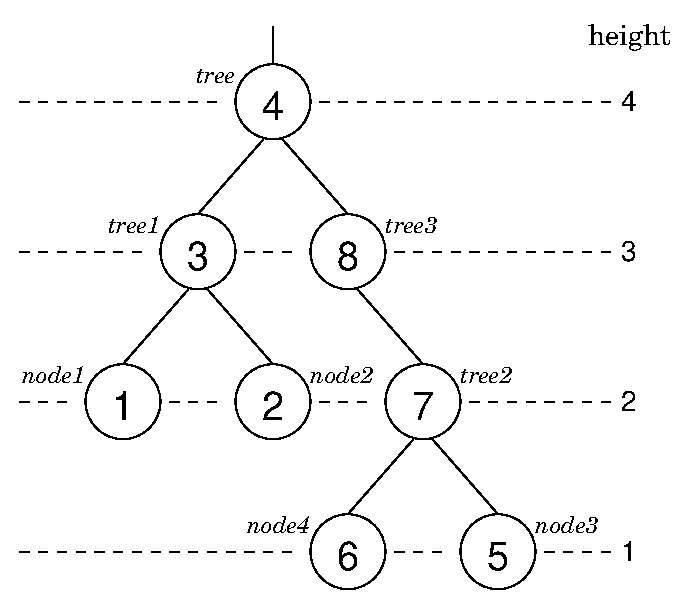
\includegraphics[height=60.0mm]{tree.eps}
\end{screen}

\newpage

\begin{flushright}
  $B>pJsDL?.9)3X<B83(BIB$BBh(B6$B=52]Bj(B
\end{flushright}

\underline{$B3X@RHV9f(B:\makebox[30.0mm]{}$B;aL>(B:\makebox[50.0mm]{}}
\vspace{5.0mm}

\begin{screen}
\end{screen}

\end{document}

